\subsection{SEMI-DIRECT PRODUCTS}

Let \(\mathfrak{a}\) and \(\mathfrak{b}\) be two Lie algebras over \(\mathbf{K}\) . It is not easy to construct all the extensions of \(\mathfrak{b}\) by \(\mathfrak{a}\) . But we shall describe quite simply all the inessential extensions of \(\mathfrak{b}\) by \(\mathfrak{a}\) .

Let \(g\) be an inessential extension of \(b\) by \(a\) . We identify \(a\) with an ideal of \(g\) , \(b\) with a subalgebra of \(g\) supplementary to \(a\) and the module \(g\) with the module \(a \times b\) . For all \(b \in b\) , let \(\phi_b\) be the restriction to \(a\) of \(ad_g b\) ; this is a derivation of \(a\) and the mapping \(b \mapsto \phi_b\) is a homomorphism of \(b\) into the Lie algebra of derivations of \(a\) . On the other hand, for \(a, a'\) in \(a\) and \(b, b'\) in \(b\) , we have:

\[
\begin{array}{r l} {[ (a, b), (a ^ {\prime}, b ^ {\prime}) ]} & {= [ a + b, a ^ {\prime} + b ^ {\prime} ]} \\ & {= [ a, a ^ {\prime} ] + [ a, b ^ {\prime} ] + [ b, a ^ {\prime} ] + [ b, b ^ {\prime} ]} \\ & {= ([ a, a ^ {\prime} ] + \phi_ {b} a ^ {\prime} - \phi_ {b ^ {\prime}} a, [ b, b ^ {\prime} ]).} \end{array}\tag{6}
\]

Conversely, let \(\mathfrak{a}\) and \(\mathfrak{b}\) be Lie algebras over \(\mathbf{K}\) and \(b \mapsto \phi_b\) a homomorphism of \(\mathfrak{b}\) into the Lie algebra of derivations of \(\mathfrak{a}\) . On the product \(\mathfrak{g}\) of the K-modules \(\mathfrak{a}\) and \(\mathfrak{b}\) we define the bracket of two elements by writing:

\[
[ (a, b), (a ^ {\prime}, b ^ {\prime}) ] = ([ a, a ^ {\prime} ] + \phi_ {b} a ^ {\prime} - \phi_ {b ^ {\prime}} a, [ b, b ^ {\prime} ])
\]

for all \(a, a'\) in \(\mathfrak{a}, b, b'\) in \(\mathfrak{b}\) . It is immediate that this bracket is an alternating bilinear function of \((a, b), (a', b')\) ; we show that, given 3 elements \((a, b), (a', b'), (a'', b'')\) of \(\mathfrak{a} \times \mathfrak{b}\) :

\[
\begin{array}{r l} {[ (a, b), [ (a ^ {\prime}, b ^ {\prime}), (a ^ {\prime \prime}, b ^ {\prime \prime}) ] ] + [ (a ^ {\prime}, b ^ {\prime}), [ (a ^ {\prime \prime}, b ^ {\prime \prime}), (a, b) ] ]} & \\ {+ [ (a ^ {\prime \prime}, b ^ {\prime \prime}), [ (a, b), (a ^ {\prime}, b ^ {\prime}) ] ] = 0.} \end{array}\tag{7}
\]

As the left hand side of (7) is an alternating trilinear function of \((a, b)\) , \((a', b')\) , \((a'', b'')\) , it suffices to make the verification when this system of elements takes one of the following forms:

\[
(a, 0), (a ^ {\prime}, 0), (a ^ {\prime \prime}, 0)\tag{8}
\]

\[
(a, 0), (a ^ {\prime}, 0), (0, b ^ {\prime \prime})\tag{9}
\]

\[
(a, 0), (0, b ^ {\prime}), (0, b ^ {\prime \prime})\tag{10}
\]

\[
(0, b), (0, b ^ {\prime}), (0, b ^ {\prime \prime})\tag{11}
\]

In cases (8) and (11), relation (7) is an immediate consequence of the Jacobi identity in a and b. In case (9), we have

\[
\begin{array}{l} [ (a, 0), [ (a ^ {\prime}, 0), (0, b ^ {\prime \prime}) ] ] = [ (a, 0), (- \phi_ {b ^ {\prime \prime}} a ^ {\prime}, 0) ] = (- [ a, \phi_ {b ^ {\prime \prime}} a ^ {\prime} ], 0) \\ {} [ (a ^ {\prime}, 0), [ (0, b ^ {\prime \prime}), (a, 0) ] ] = [ (a ^ {\prime}, 0), (\phi_ {b ^ {\prime \prime}} a, 0) ] = ([ a ^ {\prime}, \phi_ {b ^ {\prime \prime}} a ], 0) \\ {} [ (0, b ^ {\prime \prime}), [ (a, 0), (a ^ {\prime}, 0) ] ] = [ (0, b ^ {\prime \prime}), ([ a, a ^ {\prime} ], 0) ] = (\phi_ {b ^ {\prime \prime}} ([ a, a ^ {\prime} ]), 0) \end{array}
\]

and relation (7) follows from the equation:

\[
\phi_ {b ^ {\prime \prime}} ([ a, a ^ {\prime} ]) = [ \phi_ {b ^ {\prime \prime}} a, a ^ {\prime} ] + [ a, \phi_ {b ^ {\prime \prime}} a ^ {\prime} ].
\]

In case (10), we have:

\[
[ (a, 0), [ (0, b ^ {\prime}), (0, b ^ {\prime \prime}) ] ] = [ (a, 0), (0, [ b ^ {\prime}, b ^ {\prime \prime} ]) ] = (- \phi_ {[ b ^ {\prime}, b ^ {\prime \prime} ]} a, 0)
\]

\[
[ (0, b ^ {\prime}), [ (0, b ^ {\prime \prime}), (a, 0) ] ] = [ (0, b ^ {\prime}), (\phi_ {b ^ {\prime \prime}} a, 0) ] = (\phi_ {b ^ {\prime}} \phi_ {b ^ {\prime \prime}} a, 0)
\]

\[
[ (0, b ^ {\prime \prime}), [ (a, 0), (0, b ^ {\prime}) ] ] = [ (0, b ^ {\prime \prime}), (- \phi_ {b ^ {\prime}} a, 0) ] = (- \phi_ {b ^ {\prime \prime}} \phi_ {b ^ {\prime}} a, 0)
\]

and relation (7) follows from the equation:

\[
\phi_ {[ b ^ {\prime}, b ^ {\prime \prime} ]} = \phi_ {b ^ {\prime}} \phi_ {b ^ {\prime \prime}} - \phi_ {b ^ {\prime \prime}} \phi_ {b ^ {\prime}}.
\]

Hence a Lie algebra structure has been defined on g. The mapping \((a, b) \mapsto b\) of g onto b is a homomorphism \(\mu\) whose kernel n is the ideal of elements of g of the form \((a, 0)\) . The mapping \(a \mapsto (a, 0)\) is an isomorphism \(\lambda\) of a onto n.~Hence:

\[
a \xrightarrow {\lambda} g \xrightarrow {\mu} b\tag{12}
\]

is an extension of b by a of kernel n, which is said to be canonically defined by a, b, \(\phi\) . The mapping \(b \mapsto (0, b)\) is an isomorphism v of b onto a subalgebra of g supplementary to n in g; hence the extension is inessential.

If \(a\) is identified with \(n\) under \(\lambda\) and \(b\) with \(v(b)\) under \(v\) , then, for \(a \in a\) and \(b \in b\) :

\[
(\mathrm{ad} b). a = [ (0, b), (a, 0) ] = (\phi_ {b} a, 0) = \phi_ {b} a.
\]

When \(\phi = 0\) , \(\mathfrak{g}\) is the product Lie algebra of \(\mathfrak{b}\) and \(\mathfrak{a}\) . In the general case, \(\mathfrak{g}\) is called the semi-direct product of \(\mathfrak{b}\) by \(\mathfrak{a}\) (corresponding to the homomorphism \(b \mapsto \phi_b\) of \(\mathfrak{b}\) into the Lie algebra of derivations of \(\mathfrak{a}\) ).

We have therefore established the following proposition:

PROPOSITION 7. Let a and b be two Lie algebras over K,

\[
a \xrightarrow {\lambda} g \xrightarrow {\mu} b
\]

an inessential extension of b by a, v an isomorphism of b onto a subalgebra of g such that \(\mu \circ v\) is the identity automorphism of b and \(\phi\) the corresponding homomorphism of b into the Lie algebra of derivations of a. Let

\[
a \xrightarrow {\lambda_ {0}} g _ {0} \xrightarrow {\mu_ {0}} b
\]

be the inessential extension of \(\mathfrak{b}\) by a canonically defined by \(\phi\) . Then the mapping \((a, b) \mapsto \lambda(a) + v(b)\) is an isomorphism \(f\) of \(\mathfrak{g}_0\) onto \(\mathfrak{g}\) and the following diagram

\pandocbounded{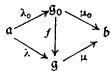
\includegraphics[keepaspectratio]{images/part001_108a7b03.jpg}}

is commutative, so that the two extensions are equivalent.

Example 1. Let g be a Lie algebra over K and D a derivation of g. Let h be the commutative Lie algebra K. The mapping \(\lambda \mapsto \lambda D (\lambda \in \mathbf{K})\) is a homomorphism of h into the Lie algebra of derivations of g. We form the corresponding semidirect product t of h by g. Let \(x_0\) be the element (0, 1) of t. For all \(x \in g\) , Dx = [x₀, x].

Example 2. Let g be a Lie algebra over K, M a K-module and \(\rho\) a homomorphism of g into gl(M). If M is considered as a commutative Lie algebra, the Lie algebra of derivations of M is gl(M). We can therefore form the semi-direct product h of g by M corresponding to \(\rho\) .

In particular, let \(\mathfrak{g} = \mathfrak{gl}(\mathbf{M})\) and \(\rho\) be the identity mapping of \(\mathfrak{gl}(\mathbf{M})\) . The semi-direct product of \(\mathfrak{g}\) by \(\mathbf{M}\) is then denoted by \(\mathfrak{af}(\mathbf{M})\) (or \(\mathfrak{af}(n,\mathbf{K})\) if \(\mathbf{M} = \mathbf{K}^{n}\) ). An element of \(\mathfrak{af}(\mathbf{M})\) is an ordered pair \((m,u)\) , where \(m\in \mathbf{M}\) , \(u\in \mathfrak{gl}(\mathbf{M})\) ; and the bracket is defined by

\[
[ (m, u), (m ^ {\prime}, u ^ {\prime}) ] = (u (m ^ {\prime}) - u ^ {\prime} (m), [ u, u ^ {\prime} ]).
\]

*When M is a finite-dimensional vector space over R, \(\mathfrak{af}(M)\) is canonically identified with the Lie algebra of the affine group of M.*

Let \(t\) be a Lie algebra over \(K\) . A linear mapping \(\theta\) of \(t\) into \(\mathfrak{af}(M)\) can be written \(x \mapsto ((\zeta(x), \eta(x))\) , where \(\zeta\) is a linear mapping of \(t\) into \(M\) and \(\eta\) a linear mapping of \(t\) into \(\mathfrak{gl}(M)\) . We examine the conditions that \(\zeta\) and \(\eta\) must satisfy for \(\theta\) to be a homomorphism. For \(x \in t, y \in t\) , we must have

\[
\theta ([ x, y ]) = [ \theta (x), \theta (y) ]
\]

that is

\[
\begin{array}{r l} (\zeta ([ x, y ]), \eta ([ x, y ])) & = [ (\zeta (x), \eta (x)), (\zeta (y), \eta (y)) ] \\ & = (\eta (x). \zeta (y) - \eta (y). \zeta (x), [ \eta (x), \eta (y) ]). \end{array}
\]

Hence for \(\theta\) to be a homomorphism of \(t\) into \(\mathfrak{af}(M)\) , it is necessary and sufficient that \(\eta\) be a homomorphism of \(t\) into \(\mathfrak{gl}(M)\) and that \(\zeta\) satisfy the relation:

\[
\zeta ([ x, y ]) = \eta (x). \zeta (y) - \eta (y). \zeta (x).\tag{13}
\]

Let \(\mathbf{N}\) be the \(\mathbf{K}\) -module \(\mathbf{M} \times \mathbf{K}\) . We take \(t\) to be the subalgebra of \(\mathfrak{gl}(\mathbf{N})\) consisting of the \(w \in \mathfrak{gl}(\mathbf{N})\) such that \(w(\mathbf{N}) \subset \mathbf{M}\) . For all \(w \in t\) , let \(\eta(w) \in \mathfrak{gl}(\mathbf{M})\) be the restriction of \(w\) to \(\mathbf{M}\) and let \(\zeta(w) = w(0,1) \in \mathbf{M}\) . For \(w_1 \in t, w_2 \in t\) ,

\[
\zeta ([ w _ {1}, w _ {2} ]) = w _ {1} (\zeta (w _ {2})) - w _ {2} (\zeta (w _ {1})) = \eta (w _ {1}). \zeta (w _ {2}) - \eta (w _ {2}). \zeta (w _ {1}).
\]

Hence the mapping \(w \mapsto (\zeta(w), \eta(w))\) is a homomorphism \(\theta\) of \(t\) into \(\mathfrak{af}(\mathbf{M})\) . Clearly \(\theta\) is bijective. Let \(\phi = \theta^{-1}\) . If \((m, u) \in \mathfrak{af}(\mathbf{M})\) , \(\phi(m, u)\) is the element \(w\) of \(t\) defined by

\[
w (m ^ {\prime}, \lambda) = (u (m ^ {\prime}) + \lambda m, 0).
\]

\(\mathfrak{af}(\mathbf{M})\) is often identified with the subalgebra \(\mathfrak{t}\) of \(\mathfrak{gl}(\mathbf{N})\) under the isomorphism \(\phi\) .

*When M is a finite-dimensional vector space over \(\mathbf{R}\) , the homomorphism \(\phi\) of \(\mathfrak{af}(M)\) into \(\mathfrak{gl}(N)\) corresponds to a canonical homomorphism \(\psi\) of the affine group A of M into the group \(\mathbf{GL}(N)\) ; if \(a \in A\) , \(\psi(a)\) is the unique element \(g\) of \(\mathbf{GL}(N)\) such that \(g(m, 1) = (a(m), 1)\) for all \(m \in M\) . This homomorphism is injective and \(\psi(A)\) is the set of automorphisms of N which leave invariant all the linear varieties of N parallel to M.*

